\documentclass[11pt,a4paper,ngerman]{article}
\usepackage[bottom=2.5cm,top=2.5cm]{geometry} 
\usepackage{babel}
\usepackage[utf8]{inputenc} 
\usepackage[T1]{fontenc} 
\usepackage{ae} 
\usepackage{amssymb} 
\usepackage{amsmath} 
\usepackage{graphicx}
\usepackage{fancyhdr}
\usepackage{fancyref}
\usepackage{listings}
\usepackage{xcolor}
\usepackage{paralist}
\usepackage{fancyhdr}
\usepackage{subfigure}
\pagestyle{fancy}
\fancyhead[C]{Mikroprozessorpraktikum}
\fancyhead[L]{Protokoll 2}
\fancyhead[R]{WS 2011/12}
\fancyfoot{}
\fancyfoot[L]{}
\fancyfoot[C]{\thepage / \pageref{LastPage}}
\renewcommand{\footrulewidth}{0.5pt}
\renewcommand{\headrulewidth}{0.5pt}
\setlength{\parindent}{0pt} 
\setlength{\headheight}{15pt}


\author{Teilnehmer:\\ \\Marco Träger, Matr. 4130515\\Alexander Steen, Matr. 4357549}
\date{Gruppe: Freitag, Arbeitsplatz: HWP 1}
\title{Mikroprozessorpraktikum WS 2011/12\\ Aufgabenkomplex: 2}

\begin{document}

\lstset{language=c, basicstyle=\ttfamily\fontsize{9pt}{9pt}\selectfont\upshape, commentstyle=\rmfamily\slshape, keywordstyle=\rmfamily\bfseries, breaklines=true, frame=single, xleftmargin=3mm, xrightmargin=3mm, tabsize=2}

\maketitle
\thispagestyle{fancy}
\newpage
\section*{A 2.1 Taktfrequenz}

\begin{description}
	\item[A 2.1.1] Bestimmen Sie messtechnisch die Frequenz der \texttt{LFXT1CLK}- und \texttt{XT2CLK}-Taktquelle. \\ \\
	Zur Lösung dieser Aufgabe werden zusätzlich zu den in Aufgabenblock 1 beschriebenen Registern das \texttt{BC2CTL2}-Register benutzt. In diesem Register werden einige der Bits für die Taktsteuerung verwaltet. Die zwei höchstwertigsten Bits legen die Taktquelle und die zwei nächst niederen Bits die Auswahl des Taktteilers fest. Für diese Aufgabe wird die Taktteilung ausgeschaltet (also auf den Divisor 1), damit der tatsächliche Takt gemessen wird.
		\begin{description}
			\item[LFXT1CLK] Um auf P5.4 das Taktsignal messen zu können, wird nach dem Verbinden der Portleitung mit dem Takt (via \texttt{P5SEL}) das Messgerät angeschaltet. Nun wird das folgende Programm ausgeführt:
\begin{lstlisting}
void aufgabe211() {
    P5SEL |= (1 << 4);	// Leitung mit Modul verbinden
    P5DIR |= (1 << 4);	// Als Ausgang fungieren
    BCSCTL2 = (BCSCTL2 & ~SELM_3) | SELM_3; // LFXTCLK
    BCSCTL2 = (BCSCTL2 & ~DIVM_3) | DIVM_0; // Divisor 1
}
\end{lstlisting}
			Am Messgerät lässt lässt sich eine Frequenz von $32,76927$ kHz messen. Dies ist die Taktfrequenz der \texttt{LFXT1CLK}.
			\item[XT2CLK]  Diese Messung wird analog zur \texttt{LFXT1CLK}-Messung durchgeführt. Einzig die Selektion der Taktquelle ändert sich (siehe Code):
\begin{lstlisting}
void aufgabe211() {
    P5SEL |= (1 << 4);	// Leitung mit Modul verbinden
    P5DIR |= (1 << 4);	// Als Ausgang fungieren
    BCSCTL2 = (BCSCTL2 & ~SELM_3) | SELM_2; // XT2CLK
    BCSCTL2 = (BCSCTL2 & ~DIVM_3) | DIVM_0; // Divisor 1
}	
\end{lstlisting}
			Aus der Messung ergibt sich eine Taktfrequenz von $7,373165$ MHz für die \texttt{XT2CLK}-Taktquelle.
		\end{description}
	

	\item[A 2.1.2] Bestimmen Sie messtechnisch die minimale und maximale Taktfrequenz des \texttt{MCLK}-Taktes, die sich auf Basis der \texttt{LFXT1CLK}-, \texttt{XT2CLK}- und \texttt{DCOCLK}-Taktquellen bereitstellen läßt. Belegen Sie die Messergebnisse mit einer Berechnung auf Basis aller Komponenten aus den Blockschaltbildern.
		
		\begin{description}
			\item[LFXT1CLK] Als maximale Frequenz dieser Taktquelle kann das Ergebnis aus Aufgabe 2.1.1 hergenommen werden, also $f_{max} \approx 32,76927 \text{ kHz }$. Durch Modifikation mit dem größten Taktteiler (ein Achtel) können wir hier den minimalen Takt $f_{min}$ produzieren. Also ergibt sich als Code:
\begin{lstlisting}
void aufgabe212() {
    P5SEL |= (1 << 4);	// Leitung mit Modul verbinden
    P5DIR |= (1 << 4);	// Als Ausgang fungieren
    BCSCTL2 = (BCSCTL2 & ~SELM_3) | SELM_3; // LFXTCLK
    BCSCTL2 = (BCSCTL2 & ~DIVM_3) | DIVM_3; // Divisor 8
}
\end{lstlisting}
			Aus der Messung ergibt sich ein Takt von $4,096158$ kHz. \\
			Dies deckt sich mit den Erwartungen, da sich für die minimale Taktfrequenz rechnerisch ergibt:
			$$ f_{min} = f_{max} \cdot \frac{1}{8} \approx 32,76927 \text{ kHz} \cdot \frac{1}{8} \approx 4,096159 \text{ kHz}$$
			
			\item[XT2CLK] Analog zur \texttt{LFXT1CLK}-Taktquelle, können wir die maximale Frequenz aus Aufgabe 2.1.1 nehmen, die minimale Frequenz wiederum durch den Taktteiler mit Divisor 8 erreichen. Der Code dazu ist ebenfalls analog, wird darum nicht wiederholt. \\ \\
			Also ergibt sich für die maximale Frequenz $f_{max} \approx 7,373165 \text{ MHz}$. \\
			Die Messung des minimalen Taktes ergibt eine Frequenz von $921,6456 \text{ kHz}$. \\
			Auch dies stimmt mit dem rechnerischen Ergebnis überein:
			$$ f_{min} = f_{max} \cdot \frac{1}{8} \approx 7,373165 \text{ MHz} \cdot \frac{1}{8} \approx 921,6456 \text{ kHz}$$
			\item[DCOCLK] Um die minimale und maximale Frequenz der \texttt{DCOCLK}-Taktquelle zu messen, binden wir in der \texttt{main.c} wieder die DCO-Quelle ein (Funktionsaufruf \texttt{DCO();}). Bei dieser Taktquelle können wir zusätzlich mit Hilfe des \texttt{DCOR}-Bits die Frequenz manipulieren. Dies kann ebenfalls im \texttt{BCSCTL2}-Register gesetzt werden. Die erste Messung wurde mit \texttt{DCOR} = 0 durchgeführt:
			\begin{lstlisting}
void aufgabe212() {
    P5SEL |= (1 << 4);	// Leitung mit Modul verbinden
    P5DIR |= (1 << 4);	// Als Ausgang fungieren
    BCSCTL2 = (BCSCTL2 & ~SELM_3) | SELM_0; // DCO
    BCSCTL2 = (BCSCTL2 & ~DIVM_3) | DIVM_0; // Divisor 1
    BCSCTL2 &= ~DCOR;  // DCOR auf 0
}
\end{lstlisting}
			Die Messung ergibt einen Takt von $ f_{DCOR = 0} \approx 1,7026 \text{ MHz} $.
			Mit gesetztem DCOR-Bit ergibt die Messung $ f_{DCOR = 1} \approx 7,3684 \text{ MHz} $, was also die maximale Frequenz $f_{max}$ ist. \\
			Für die Messung der minimalen Frequenz wird der Taktteiler wie in den vorigen Aufgaben genutzt, deshalb wird der Code nicht gezeigt. Die Messung für die minimale Frequenz ergibt einen Takt von ca. $212,8 \text{ kHz}$. Dies bestätigt das rechnerische Ergebnis:
			$$ f_{min} = f_{DCOR = 0} \cdot \frac{1}{8} \approx 1,7026 \text{ MHz} \cdot \frac{1}{8} = 212,825 \text{ kHz} $$
		\end{description}
		
	\item[A 2.1.3] An P2.5 ist ein Oszillatorwiderstand $R_{osc}$ von 39kOhm angeschlossen. Erläutern Sie, wie der externe Widerstand für den \texttt{DCOCLK}-Taktgenerator nutzbar gemacht wird. \\
		
		Der externe Oszillatorwiderstand kann mit Hilfe des \texttt{DCOR}-Bits über das \texttt{BCSCTL2}-Register dazugeschaltet werden. Ist das Bit auf Eins geschaltet, wird der externe Widerstand genutzt.	
		
	\item[A 2.1.4] Welchen Einfluss hat der Widerstand auf den \texttt{DCOCLK}-Taktgenerator?  \\
	
	Bei der Auswahl des Oszillatorwiderstands via \texttt{DCOR}-Bit wird die Taktfrequenz größer. Wie man aus der Tabelle aus Aufgabe A 2.2.1 entnehmen kann, ist bei gleichem Divisor der Takt mit gewähltem Oszillatorwiderstand (ganz grob) vier Mal größer als ohne. \\
Dies wird wohl daher kommen, dass der Oszillatorwiderstand zusätzlich zum Taktgenerator schwingt und mit dem Takt positiv interferiert, sodass sich beide Takte zu einem größeren Takt ergänzen.

\end{description}

\newpage
\section*{A 2.2 Stromverbrauch}

\begin{description}
	\item[A 2.2.1] Der \texttt{MCLK}-Takt soll durch den \texttt{DCOCLK}-Taktgenerator bereitgestellt werden. Ermitteln Sie für diesen Fall die Abhängigkeit des Stromverbrauchs von der Taktfrequenz. Stellen Sie die Abhängigkeit für einen Bereich von 100kHz bis 10MHz grafisch dar. 
	
	Die gemessenen Ströme sind wie folgt: \\
	\begin{tabular}{c|c|c|c}
	  \texttt{DCOR} & Divisor & Frequenz [Hz]  & Strom [mA]) \\
	\hline \hline
		0&	8&	212,49 $\cdot 10^3$&	1,18 \\
		0&	4&	426,35 $\cdot 10^3$&	1,30 \\
		0&	2&	852,32 $\cdot 10^3$&	1,55 \\
		0&	1&	1,703 $\cdot 10^6$	&	2,19 \\
		1&	8&	926,74 $\cdot 10^3$&	1,87 \\
		1&	4&	1,852 $\cdot 10^6$	&	2,41 \\
		1&	2&	3,702 $\cdot 10^6$	&	3,46 \\
		1&	1&	7,371 $\cdot 10^6$	&	6,16 \\
	\end{tabular}
	\\ \\ \\
	Dann ergibt sich als Abhängigkeit zwischen Frequenz und Stromverbrauch:
	\begin{figure}[h!]
			\hspace{1cm}
			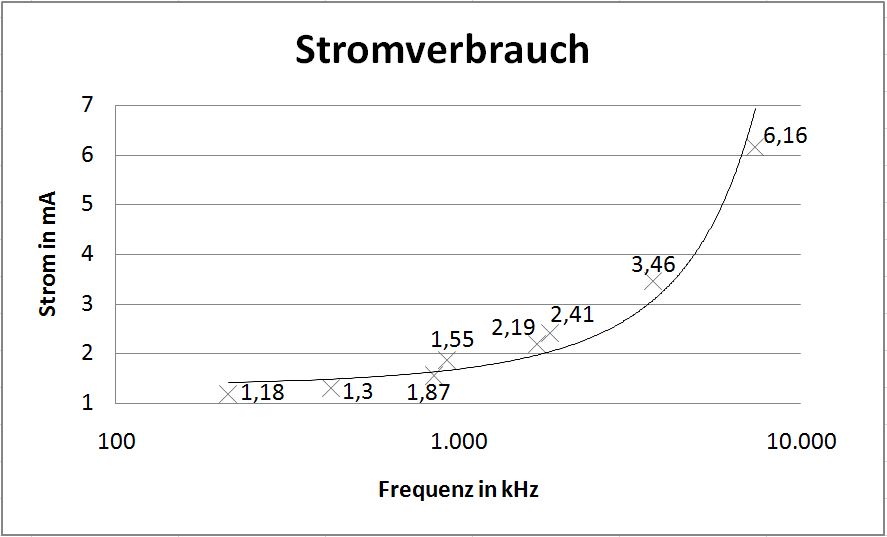
\includegraphics[scale=0.5]{stromverbrauch.png}
		\end{figure}
		\\
	Die durchgezogene Linie stellt eine exponentielle Ausgleichskurve dar.
\end{description}

\pagebreak
\section*{A 2.3 Taktumschaltung}
\begin{description}
\item[A 2.3.1] Entwickeln Sie ein Programm, das auf Tastendruck die Taktfrequenz des Mikrocontrollers zwischen 4,096kHz und 7,3728 MHz umschaltet. \\

Das nachfolgende Programm schaltet bei einem Druck auf die rechte Taste die Taktfrequenz auf 4,096 kHz und bei einem Druck auf die linke Taste auf 7,3728 MHz.
\begin{lstlisting}[numbers=left]
// Initialisierung der Register
// wird nicht in der while-Schleife
// aufgerufen.
init231() {
	// alle LEDs ausschalten
	// und Register korrekt setzen
	P4SEL &= ~(0x07); // I/O Funktion
	P4DIR |= 0x07; // Output
	P4OUT |= 0x07; // Alle LEDs
	LEDOFF;		   // aus

	// Schalter einrichten
	P1SEL &= ~(0x03); // I/O Funktion
	P1DIR &= ~(0x03); //Input

	// Taktfrequenzen erreichbar:
	// 4,096kHz mit LFXTCLK Divisor /8
	// 7,3728 MHz mit DCO Divisor /1 und DCOR 1

	// Output des Takts
	P5SEL |= (1 << 4);
	P5DIR |= (1 << 4);
}	
// Hauptprogramm
void aufgabe231() {
	if (P1IN & 0x01) // rechte Taste gedrueckt
	{
			BCSCTL2 = (BCSCTL2 & ~SELM_3) | SELM_3; // LFXTCLK
			BCSCTL2 = (BCSCTL2 & ~DIVM_3) | DIVM_3; // Divisor 8
	}
	if (P1IN & 0x02) // linke Taste gedrueckt
	{
			// DCO
			BCSCTL2 = (BCSCTL2 & ~SELM_3) | SELM_0; // DCO
			BCSCTL2 = (BCSCTL2 & ~DIVM_3) | DIVM_0; // Divisor 1
			BCSCTL2 |= DCOR;  // DCOR auf 1
	}
}
\end{lstlisting}

Bei den Messungen ergibt sich für die Frequenz $7,347$ MHz ein Stromverbrauch von ca. $4,87$ mA. Bei einer Taktfrequenz von $4,096$ kHz wurde ein Stromverbrauch von ca. $0,491$ mA gemessen.

\item[A 2.3.2] Welche Schlußfolgerungen hinsichtlich des Energieverbrauches ziehen Sie? Berechnen Sie für beide gemessenen Stromverbrauchswerte die theoretisch mögliche Batterielaufzeit des MSB430H bei Nutzung einer Batterie mit einer Kapazität von 1100mAh. \\

Da der Energieverbrauch bei höheren Taktfrequenzen schnell ansteigt, sollte man den Takt nach Möglichkeit gering halten, um so die Batterielaufzeit zu optimieren.\\
Die Lebensdauer $t$ einer Batterie lässt sich durch die Formel 
$$ t = \frac{\text{Kapazität}}{\text{Verbrauch}} $$
bestimmen. 
\newpage
Bei einer Batterie mit einer Kapazität von $1100 \; mAh$ ergibt sich dann für einen Takt von 4,096 kHz:
$$ t = \frac{1100 \; mAh}{0,491 \; mA} = 2240 \; h \approx 3,07 \; \text{Monate}$$
Und für den Takt von 7,347 MHz:
$$ t = \frac{1100 \; mAh}{4,87 \; mA} = 225,9 \; h \approx 9,41 \; \text{Tage} $$

Bei der niedrigeren Frequenz kann das Modul also ca. drei Monate mit einer Batterieladung auskommen, bei der höheren Frequenz allerdings nur ca. 9 Tage.

\end{description}

\section*{A 2.4 Codezeile}
\begin{description}
\item[A 1.4.1]Bestimmen Sie messtechnisch die Abarbeitungzeit von \texttt{P5OUT \textasciicircum = 0x10;} bei Nutzung der \texttt{XT2CLK} und der \texttt{LFXT1CLK} Taktquelle. \\

Bei diesem Programm wird das Ausgangssignal periodisch invertiert, sodass der Signalwechsel via Messgerät erfassbar wird:

\begin{lstlisting}[numbers=left]
	// Output des Takts
	P5SEL &= ~(1 << 4);
	P5DIR |= (1 << 4);
	// Taktquelle einstellen
	BCSCTL2 = (BCSCTL2 & ~SELM_3) | SELM_3; // LFXTCLK
	BCSCTL2 = (BCSCTL2 & ~DIVM_3) | DIVM_0; // Divisor 1
	// Signal invertieren
	while(1)
	{
		P5OUT^= 0x10;
	}
\end{lstlisting}  
Dieses Programm löst die Aufgabe für die \texttt{LFXT1CLK}-Clock; das Programm für \texttt{XT2CLK} ist analog - hier wird nur eine andere Taktquelle ausgewählt.\\
Dann ergibt sich für die Messungen:
\begin{description}
\item[LFXT1CLK] Gemessene Frequenz $f$ am Port: ca. 2,34 kHz \\
Die Periodenlänge $T$, die die Länge eines $0 \rightarrow 1 \rightarrow 0$-Durchlaufs angibt, ergibt sich via Formel $T = \frac{1}{f}$, also ist
$$ T = \frac{1}{f} = \frac{1}{2,34 \; kHz} = 427.4 \; \mu s $$.
Die Abarbeitung des Befehls entspricht genau den halben Periodenlänge der Schwingung. Also dauert die Abarbeitung des Befehls ungefähr $213.7 \; \mu s$.

\item[XT2CLK] Gemessene Frequenz $f$ am Port: ca. 526,65 kHz \\
Die Abarbeitungzeit $D$ ergibt sich analog.
$$ D = \frac{1}{2} T = \frac{1}{2 f} = \frac{1}{2 \cdot 526,65 \; kHz} = 949,4 \;  ns  $$
Also dauert die Abarbeitung des Befehls ungefähr $949,4 \;  ns$.
\end{description}     
\end{description}
\label{LastPage}
\end{document}